\documentclass[../PhysicsFormulae]{subfiles}
\begin{document}

\subsection{Kirchhoff's Laws}
Because charge must be conserved, at any junction, the total input current must equal the total output current. This is known as Kirchhoff's Current Law, or KCL. \bigskip

Because energy must be conserved, around a closed loop, sum of all electric potentials must be 0. This is known as Kirchhoff's Voltage Law, or KVL. 

\subsection{Electromotive Force}
The emf is defined as the work per unit charge done in a circuit by any component, or 
\[ \varepsilon = \frac{dW}{dq} \]
It is analagous to a pump in fluid flow, which maintains a pressure difference between two points. Note that the emf does not supply charge to a circuit; it simply increases pumps energy into it by (usually) elevating electrons to a lower potential. \bigskip

The emf can also be expressed as 
\[ \varepsilon = \oint \frac{\vec{F}}{q} \cdot d\vec{s} \]
Generally, $\vec{F}/q$ may not equal $\vec{E}$ because the work done might be mechanical, chemical, thermal, or magnetic in nature. \bigskip

Oftentimes, the emf is provided by a battery which has internal resistance. Because the current is $i = \varepsilon / (R + r)$, where $r$ is the internal resistance and $R$ is the resistance of the rest of the circuit, the effective voltage provided by the battery is 
\[ \Delta V = \varepsilon - ir = \varepsilon \frac{R}{R+r} \]

\subsection{Voltage Divider}
A common way to obtain a lower voltage is by connecting two resistors in series and putting an output path between them. Suppose the resistors are $R_1$ and $R_2$, with the divider coming after the first resistor. Then 
\[ V_{out} = \frac{R_2}{R_1 + R_2} V_{in} \]

\subsection{Resistors in Series and Parallel}
Resistors in parallel share the same voltage drop across them, no matter the physical appearance of their arrangement. The equivalent resistance is then 
\[ R_{eq} = \cfrac{1}{\frac{1}{R_1} + \frac{1}{R_2} + \cdots + \frac{1}{R_N}} \]
Resistors in series share the same current through them. The equivalent resistance is 
\[ R_{eq} = R_1 + R_2 + \cdots + R_N \]

Probably one of the most useful techniques for solving resistors problems is that equipotential points can be connected by a wire without changing the circuit. This is because no charge will ``flow'' between two regions of same potential, but connecting them with a wire may allow us to cordon off a part of the circuit that we can apply series/parallel resistor rules to. Symmetry considerations are also supremely useful for circuits in general; for instance, two points are at equipotential if they are on opposite sides of a symmetrical circuit. 

\subsection{Energy Transfers in a Circuit}
The power delivered by a battery is 
\[ P_{emf} = \frac{dW}{dq} \frac{dq}{dt} = \varepsilon i \]
For a resistor, the power dissipated is 
\[ P = i \Delta V_R = \frac{\Delta V_R^2}{R} = i^2 R \]
where $\Delta V_R$ is the voltage across the resistor. This energy transfer to a resistor is known as \textit{Joule heating}. 

\subsection{RC Circuits}
By applying KVL to an RC circuit, we obtain a differential equation that can be solved for current and capacitor charge as a function of time. While charging the capacitor, we have 
\[ \varepsilon - iR - \frac{q}{C} = 0 \]
which yields, after substituting $i = dq/dt$, 
\[ q = C\varepsilon (1 - e^{-t/RC} ) \]
\[ i = \frac{\varepsilon}{R}e^{-t/RC} \]
where the \textit{capacitive time constant} of the circuit is $\tau_C = RC$. 

\begin{figure}[h]
	\centering
	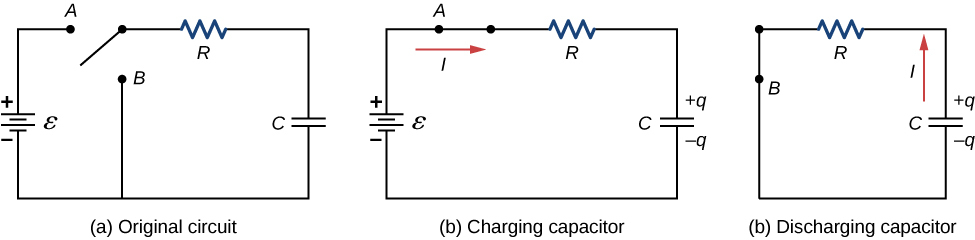
\includegraphics[width=0.7\linewidth]{images/27.rc_circuit.jpg}
	\caption{Charging and discharging an RC circuit}
\end{figure}

While discharging the capacitor, we have 
\[ \frac{q}{C} - iR = 0 \]
which yields 
\[ q = q_0 e^{-t/\tau_C} \]
\[ i = -\frac{q_0}{RC}e^{-t/\tau_C} \]
If the capacitor was fully charged at $q_0 = \epsilon C$, then the current function reduces down to
\[ i = -\frac{\varepsilon}{R}e^{-t/\tau_C} \]

\end{document}